\documentclass[a4paper]{article}

% CJK support: prefer ctex, fallback to XeTeX native line breaking
\IfFileExists{ctex.sty}{
  \usepackage[fontset=fandol]{ctex}
}{
  % Fallback for minimal TeX installs (e.g. MacTeX Basic, TeX Live scheme-basic)
  % without ctex/xeCJK. Uses XeTeX's built-in CJK line breaking.
  \usepackage{fontspec}
  \XeTeXlinebreaklocale "zh"
  \XeTeXlinebreakskip = 0pt plus 1pt
  \IfFontExistsTF{Songti SC}{\setmainfont{Songti SC}}{%
    \IfFontExistsTF{Noto Serif CJK SC}{\setmainfont{Noto Serif CJK SC}}{}%
  }
  \IfFontExistsTF{Heiti SC}{\setsansfont{Heiti SC}}{%
    \IfFontExistsTF{Noto Sans CJK SC}{\setsansfont{Noto Sans CJK SC}}{}%
  }
}

% Basic packages
\usepackage{amsmath, amssymb}
\usepackage{graphicx}
\usepackage[margin=2.5cm]{geometry}
\usepackage[most]{tcolorbox}
\usepackage{etoolbox}
\usepackage{listings}
\usepackage{hyperref}
\hypersetup{hidelinks,pdftitle={南京大学生成式软件工程第8讲：Agent-native开发},pdfauthor={lecture-to-notes}}
\usepackage{booktabs}
\usepackage{subcaption}
\usepackage{float}
\usepackage{tikz}
\IfFileExists{pgfplots.sty}{
    \usepackage{pgfplots}
    \pgfplotsset{compat=1.18}
}{}

% ===== Highlight boxes =====
\newtcolorbox{knowledgebox}[1]{
    enhanced, colback=black!2!white, colframe=black!65, colbacktitle=black!65,
    coltitle=white, fonttitle=\bfseries, title=#1, attach boxed title to top left={yshift=-2mm, xshift=2mm},
    boxrule=1pt, sharp corners
}

\newtcolorbox{importantbox}[1]{
    enhanced, colback=red!3!white, colframe=red!45!black, colbacktitle=red!45!black,
    coltitle=white, fonttitle=\bfseries, title=#1, sharp corners
}

\newtcolorbox{warningbox}[1]{
    enhanced, colback=red!5!white, colframe=red!75!black, colbacktitle=red!75!black,
    coltitle=white, fonttitle=\bfseries, title=#1, sharp corners
}

% ===== Code listings =====
\lstset{
    basicstyle=\ttfamily\small,
    keywordstyle=\color{blue},
    stringstyle=\color{red!60!black},
    commentstyle=\color{green!60!black},
    breaklines=true,
    frame=single,
    numbers=left,
    numberstyle=\tiny\color{gray},
    captionpos=b,
    extendedchars=false
}

% ===== Figure provenance and unit macros =====
% \vtag goes inside \caption{...}; \srcnote{MM:SS--MM:SS} follows the figure environment.
\newcommand{\vtag}{\protect\footnotemark}
\newcommand{\srcnote}[1]{\footnotetext{视频画面时间区间：#1。若为裁剪图，时间区间仍对应原视频画面。}}
% Units work in text and math mode; never hand-write $^\circ$ or \AA inside \mathrm.
\newcommand{\degC}{\ensuremath{^{\circ}\mathrm{C}}}
\newcommand{\um}{\ensuremath{\mu\mathrm{m}}}
\newcommand{\nm}{\ensuremath{\mathrm{nm}}}
\newcommand{\angstrom}{\ensuremath{\text{\AA}}}

% ===== Front-page metadata =====
% Fill these in when generating notes.
\newcommand{\notetitle}{Agent-native 开发}
\newcommand{\notesubtitle}{南京大学生成式软件工程 · 第 8 讲}
\newcommand{\noteauthors}{中文课程讲义 · lecture-to-notes}
\newcommand{\notedate}{2026 年 10 月 13 日}
\newcommand{\videochannel}{蒋炎岩主讲 / 绿导师原谅你了上传}
\newcommand{\videopublishdate}{20261013}
\newcommand{\videoduration}{97 分 10 秒}
\newcommand{\videourl}{https://www.bilibili.com/video/BV11LWw6VEHW/}
\newcommand{\videocoverpath}{cover.jpg}

\begin{document}

% ===== Title page =====
\begin{titlepage}
\centering
{\Large 课程笔记\par}
\vspace{1.2cm}
{\huge\bfseries \notetitle\par}
\ifdefempty{\notesubtitle}{}{
\vspace{0.3cm}
{\large \notesubtitle\par}
}
\vspace{0.5cm}
{\large \noteauthors\par}
\vspace{0.3cm}
{\large \notedate\par}
\vspace{1.0cm}

\ifdefempty{\videocoverpath}{
{\small 请在生成笔记时填入视频封面图的本地路径。\par}
}{
\includegraphics[width=0.82\textwidth,height=0.40\textheight,keepaspectratio]{\videocoverpath}\par
}

\vfill
\begin{tcolorbox}[width=0.9\textwidth, colback=black!2!white, colframe=black!60, sharp corners]
\textbf{视频作者/频道}：\videochannel\par
\textbf{发布日期}：\videopublishdate\par
\textbf{视频时长}：\videoduration\par
\textbf{视频链接}：
\ifdefempty{\videourl}{
未填写
}{
\href{\videourl}{\nolinkurl{\videourl}}
}
\end{tcolorbox}
\end{titlepage}

\tableofcontents
\newpage

\section*{读这份讲义，先抓住什么}
AI 能很快写出一个程序，但一个程序能运行，与一个项目能继续维护，是两个验收问题。本讲讨论的是后者：怎样安排任务、保存进展、观察行为、拦住不合适的改动，让下一轮开发接得住上一轮的工作。\textbf{Agent-native 开发}在这里指从项目开始就把能读写文件、执行命令的 Agent 当作实际开发者，为它安排工作环境、约束和反馈。

阅读时可以沿着三条线索走。第一条是循环：模型怎样请求工具，长任务怎样分成多轮。第二条是门控：在哪些状态变化之前必须检查，失败以后由谁修正。第三条是关系：代码、文档、接口、译文和设计决定怎样保持一致。三条线索最终都回到同一个问题：一次开发留下的状态，能否成为下一次开发可靠的起点？

本讲义依据课堂视频、B站自动字幕和视频中的课件及现场代码整理。字幕中的 Agent、Ralph Loop、工具调用等术语按画面校正。配图的脚注给出原视频时间区间；代码摘录用于解释课堂机制，不是一套可以直接投入生产的 Agent。课堂中的仓库分析包含 Agent 现场生成的摘要，相关结构和历史按课堂展示描述，没有将这些摘要当作独立的仓库审计。对模型、教育和就业的预测保留讲者身份与不确定性。

讲者蒋炎岩；上传频道“绿导师原谅你了”。来源：\href{https://www.bilibili.com/video/BV11LWw6VEHW/}{第 8 讲课堂实录}、\href{https://jyywiki.cn/GSE/2026/}{官方课程入口}与\href{https://jyywiki.cn/GSE/2026/lect8.md}{官方第 8 讲讲义}。主体解释来自课堂视频，官方入口用于核对讲次与主题。

\section{为什么还没想清楚，也应当做一个原型}
\label{sec:prototype}
原型的价值是让设计假设遇到现实。需求和架构讨论帮助我们缩小选择范围，运行一个版本则让我们看到纸面讨论遗漏的行为。两种工作需要往返进行：原型暴露问题后，下一步可能是修改代码，也可能是重新解释需求或改变架构。

\subsection{同一个目标，可以通向很多种实现}
软件开发常从一个人的意图出发。意图需要写成可以讨论的规格，规格再变成程序。课堂将这三层称为 Intent、Spec 和 Implementation。它们之间存在一对多关系：同一个目标可以写出不同的规格，同一份规格也可以采用不同的数据表示、模块分工和实现技术。图中的板书把这种选择画成逐渐展开的路径。

\begin{figure}[H]
\centering
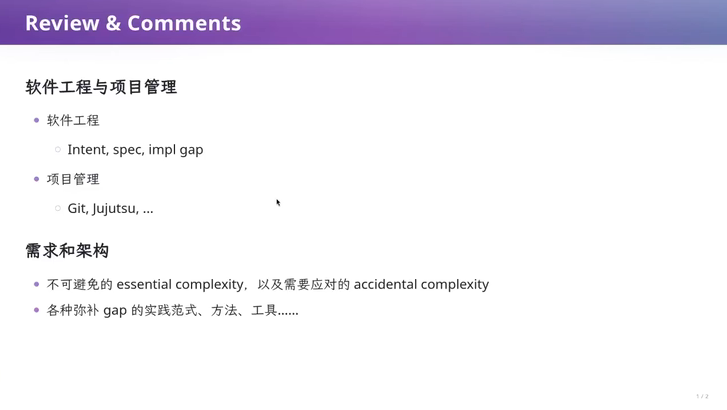
\includegraphics[width=0.98\textwidth,height=0.42\textheight,keepaspectratio]{figures/fig_01_intent_spec.png}
\caption{意图、规格、实现之间的选择空间\vtag}
\end{figure}
\srcnote{00:07:00--00:07:15}
\begin{figure}[H]
\centering
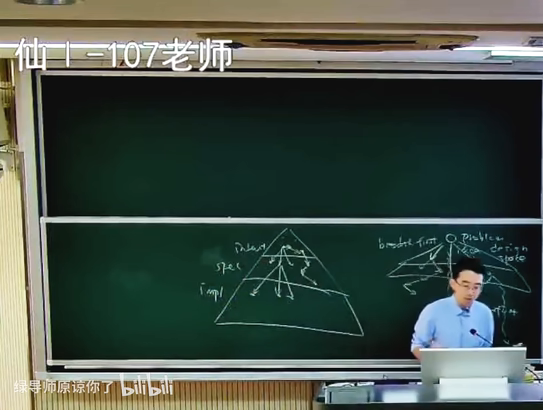
\includegraphics[width=0.98\textwidth,height=0.42\textheight,keepaspectratio]{figures/fig_02_design_space.png}
\caption{板书中的多条设计路径\vtag}
\end{figure}
\srcnote{00:07:00--00:07:15}

这解释了为什么“先想到一种办法，然后一直做下去”会有风险。沿着一条路线不断完善，是向设计空间深处探索；回到较早的岔路比较其他方案，是横向探索。深挖能得到运行结果，横向比较能发现当前路线原本就不合适。两者都消耗时间与算力，工程工作需要决定什么时候继续、什么时候返回。

\begin{importantbox}{先区分问题带来的复杂性与工具带来的复杂性}
需求本身带来的困难不会因换一个工具而消失。表示方式、实现技术和协作流程额外引入的困难，则可能通过更合适的架构减轻。课堂用本质复杂性与偶然复杂性解释这一区分。
\end{importantbox}

\subsection{评审的作用，是让早期选择有机会改变}
讲者在实验讨论中提出，Agent 往往很快选择一条看似合理的路线，然后不断向下推进。让不同模型互相评审，可能引入不同的偏见与问题意识，使早期选择重新展开。这是课堂分享的实践观察，不能据此断言任意双模型组合都优于单模型。

个人资料数据库也不足以支持所有研究任务。课堂的第二个实验把材料范围扩展到论文、博客、项目和书中片段，并要求学生观察 Agent 的行动轨迹。积累资料的意义在于给设计选择提供证据；材料只有真正影响下一步判断时，才成为研究和开发的资源。

\subsection{让失败指出应该改变哪一层}
课堂说“Let it fail”，是让一个符合当前规格的原型接受检查。程序没有按规格工作，是实现问题；规格没有表达人的需要，是需求问题；规格中的环境假设不成立，则可能需要改变设计。比如用户增多、模块发生未预见的交互，这些问题经常要在系统运行后才显现。

\begin{figure}[H]
\centering

\includegraphics[width=0.98\textwidth,height=0.42\textheight,keepaspectratio]{figures/fig_03_prototype.png}
\caption{原型检验规格中的假设\vtag}
\end{figure}
\srcnote{00:10:30--00:10:45}

课件用莱特兄弟的滑翔机说明假设也会失效：1901 年的试验中，升力只达到预测的约三分之一，失败推动他们重新检查设计数据。这里保留的是课件的教学例子，不能把“做出原型”理解为“原型一定会证实我们”。原型首先提供可以观察和比较的结果。

\begin{warningbox}{不要用一次运行替代需求验收}
“已经跑起来”只能回答特定运行条件下发生了什么。下一轮还要比较输出与规格，并检查规格依赖的使用场景、规模和环境。否则快速生成的功能可能掩盖最需要检验的假设。
\end{warningbox}

\subsection{本章小结}
开发是一连串选择，原型把选择的后果显现出来。Agent 降低了试做一个版本的成本，人的职责随之转向判断结果是否推进了目标。要让原型继续演化，先要理解 Agent 怎样通过工具改变工作区。

\section{一个最小 Agent，怎样真正执行任务}
\label{sec:inner}
Agent 与只回答文本的问题系统之间，多了一条能改变环境的通路：模型提出工具调用，普通程序执行工具，再把结果交还模型。课堂通过约 150 行的 Python 原型展示这条通路，核心机制比一个完整产品小得多。

\subsection{工具声明告诉模型，什么操作可以提出}
原型提供一个 Bash 工具。工具声明包含名称、说明和参数结构，要求模型提交一个字符串类型的 command。模型生成符合这个结构的调用，执行程序才知道应当运行哪条命令。画面中的声明可以作为一个小型接口规格来读：模型不能只说“我做过了”，它需要提出可以执行的操作。

\begin{figure}[H]
\centering
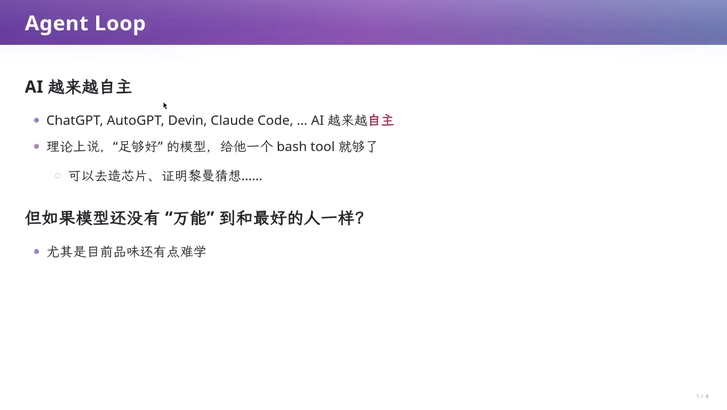
\includegraphics[width=0.98\textwidth,height=0.42\textheight,keepaspectratio]{figures/fig_04_agent_limits.png}
\caption{自主工具使用与工程品味的边界\vtag}
\end{figure}
\srcnote{00:12:00--00:12:15}
\begin{figure}[H]
\centering
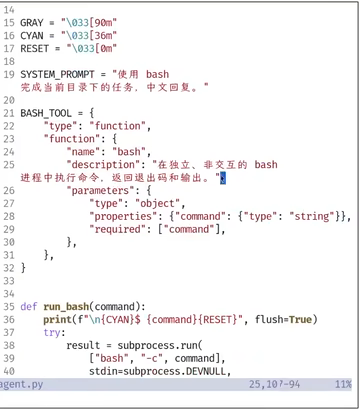
\includegraphics[width=0.98\textwidth,height=0.65\textheight,keepaspectratio]{figures/fig_05_bash_schema.png}
\caption{Bash工具的函数声明与command参数\vtag}
\end{figure}
\srcnote{00:16:30--00:16:45}

讲者提出一个思想实验：若模型足够聪明，又有充分工具和资源，单独一个 Bash 入口可能让它组织非常复杂的任务。造芯片、证明黎曼猜想在课堂中是能力想象，前提是一个尚未实现的足够强模型。现实模型仍会受既有代码影响，也会在设计品味和任务选择上偏离人的期待。

\begin{importantbox}{模型与执行程序分别负责什么}
模型选择下一步并生成工具参数；执行程序解析参数、调用工具、收集结果，并维持消息协议。工具真的运行了，才会产生文件、命令输出或其他环境变化。模型的自然语言陈述不能替代这条执行链。
\end{importantbox}

\subsection{一次工具执行，必须把失败也返回来}
课堂原型用子进程运行 Bash，把标准错误并入标准输出，记录返回码，并设置 60 秒超时。下面按屏幕中的实现摘录主要行为，省略颜色输出与界面部分：

\begin{lstlisting}[language=Python,caption={课堂原型中的命令执行与结果收集}]
result = subprocess.run(
    ["bash", "-c", command],
    stdin=subprocess.DEVNULL,
    stdout=subprocess.PIPE,
    stderr=subprocess.STDOUT,
    text=True,
    errors="replace",
    timeout=60,
)
output = f"exit_code: {result.returncode}\n{result.stdout}"
\end{lstlisting}

\begin{figure}[H]
\centering
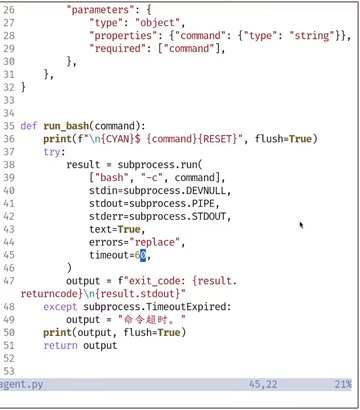
\includegraphics[width=0.98\textwidth,height=0.65\textheight,keepaspectratio]{figures/fig_06_timeout.png}
\caption{命令执行、输出收集与60秒超时\vtag}
\end{figure}
\srcnote{00:17:30--00:17:45}

返回码与错误输出让模型判断命令有没有成功。超时则显现原型与产品的差距：固定阈值在课堂机器上可能合理，网络较慢或任务较长时却可能提前终止正常工作。讲者用不同网络环境中的下载体验解释这一点。一个产品需要考虑等待、继续执行和恢复等行为，不能把某台机器上的经验当作所有环境的规格。

\subsection{工具结果怎样成为下一次推理的输入}
消息列表先包含系统说明与用户任务。模型回复后，如果没有工具调用，内循环就结束；若有调用，执行程序取出参数、运行工具，再加入角色为 tool 的结果消息。结果中的 tool\_call\_id 对应原调用的编号，使模型知道这份输出回答的是哪一次请求。

\begin{figure}[H]
\centering
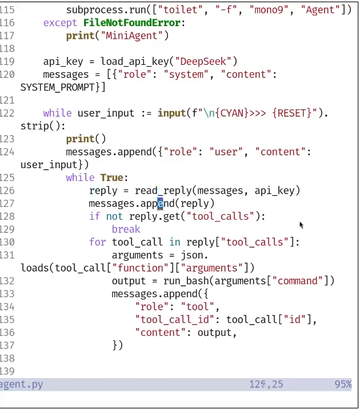
\includegraphics[width=0.98\textwidth,height=0.65\textheight,keepaspectratio]{figures/fig_07_tool_loop.png}
\caption{工具调用回写与tool\_call\_id配对\vtag}
\end{figure}
\srcnote{00:18:30--00:18:45}

\begin{lstlisting}[language=Python,caption={按课堂代码摘录的工具结果回写协议}]
while True:
    reply = read_reply(messages, api_key)
    messages.append(reply)
    if not reply.get("tool_calls"):
        break
    for tool_call in reply["tool_calls"]:
        arguments = json.loads(tool_call["function"]["arguments"])
        output = run_bash(arguments["command"])
        messages.append({
            "role": "tool",
            "tool_call_id": tool_call["id"],
            "content": output,
        })
\end{lstlisting}

\begin{warningbox}{有工具，不等于工具使用符合人的意图}
现场生成 HTML 卡片时，模型自己选择打开浏览器、检查截图并询问用户。某些行为有用，某些行为却打断了讲者希望持续推进的任务。围绕模型安排的工具、权限、流程和反馈，决定了这些行为能否用于当前工作。
\end{warningbox}

\subsection{本章小结}
内循环解决“怎样执行下一步”：模型请求工具，程序执行，结果回写。它还没有解决长任务的交接、进度判断和停止条件。接下来需要一层围绕工作区状态运行的循环。

\section{长任务怎样跨越多轮会话继续工作}
\label{sec:outer}
长任务需要保存的内容远多于当前聊天记录。代码、需求、测试、失败原因和下一步都要成为下一轮能读取的状态。外层循环重新启动会话，但保留工作区，使同一个目标可以在不同轮次中逐步推进。

\subsection{同一个提示词，为什么会产生新的进展}
课堂介绍 Ralph Loop：重复把同一份任务文本交给 Agent。名称借自《辛普森一家》中笨拙却不放弃的 Ralph。机制由三行 Shell 表达：

\begin{lstlisting}[language=bash,caption={课件中的 Ralph Loop 骨架}]
while true; do
    cat PROMPT.md | claude -p
done
\end{lstlisting}

\begin{figure}[H]
\centering
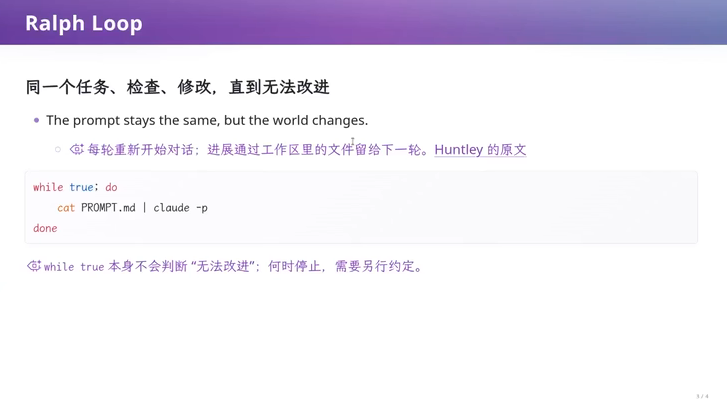
\includegraphics[width=0.98\textwidth,height=0.42\textheight,keepaspectratio]{figures/fig_08_ralph.png}
\caption{重复同一提示词的三行Ralph循环\vtag}
\end{figure}
\srcnote{00:23:30--00:23:45}

提示词可以不变，工作区会变化。上一轮可能增加了实现、跑出失败日志、修改了待办事项；下一轮读取这些文件后，就从不同起点开始。同样的指令是在作用于不同状态，并非要求模型不断重复相同答案。

\begin{importantbox}{工作区承担协作状态}
把工作区理解为状态，把一次 Agent 工作理解为状态迁移。状态包含需求、文档、代码、测试、日志与待办。长期任务能否继续，取决于下一轮能否从留下来的材料恢复判断。
\end{importantbox}

\begin{figure}[H]
\centering
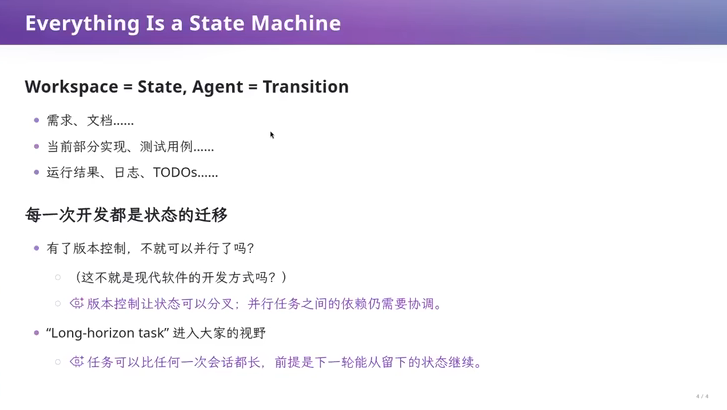
\includegraphics[width=0.98\textwidth,height=0.42\textheight,keepaspectratio]{figures/fig_09_workspace.png}
\caption{工作区状态、状态迁移与长任务\vtag}
\end{figure}
\srcnote{00:28:00--00:28:15}

\subsection{每轮留下什么，下一轮才不会重新猜}
现场循环的要求是先检查当前状态，只推进一个明确步骤，然后验证结果。未完成时，在文件里写清下一步；确认整个任务完成后，再输出约定的完成标记。课堂使用 RALPH\_DONE 一类标记让外层脚本退出。标记只是一种协议，是否应当输出仍依赖任务验收。

一份有用的交接材料应让接手者区分目标、已观察的结果和待处理问题。只写“功能已完成”，下一轮不知道通过了哪些检查；若留下失败位置与对应日志，下一轮就能继续定位。写文档的意义是恢复判断，不是展示本轮工作量。

课堂提到上下文压缩后可能丢失重要信息，也提到 500K 规模的上下文更新。这些属于授课时的产品观察。更大的窗口能容纳更多材料，但不能代替清楚的状态组织；模型换代以后，旧提示词与旧技能也应重新比较。

\subsection{版本管理让状态可以分叉，也让集成成为责任}
当状态放在 Git 或 Jujutsu 管理的工作区中，不同分支可以分别探索。图中的板书把模块 A、模块 B 的工作画成分叉，之后再合并。分叉让并行成为可能，合并仍需检查两份修改一起运行的行为。

\begin{figure}[H]
\centering
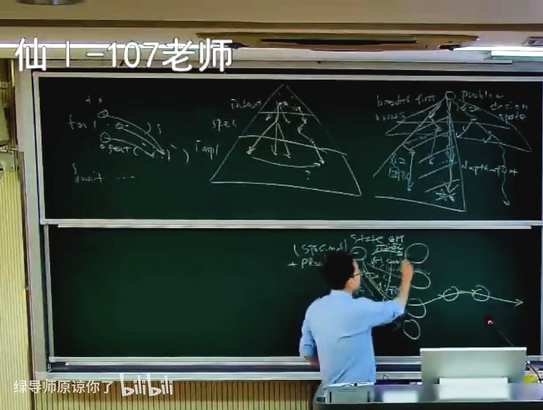
\includegraphics[width=0.98\textwidth,height=0.42\textheight,keepaspectratio]{figures/fig_10_parallel_board.png}
\caption{板书中的分支、并行修改与集成\vtag}
\end{figure}
\srcnote{00:31:00--00:31:15}

\subsection{名片演示：样式更丰富，事实未必更准确}
课堂让一次性 Agent 与外层循环完成同类名片任务。一次生成的页面有较多视觉效果，却包含错误邮箱与身份；循环生成的版本朴素一些，但讲者核对后指出邮箱和 GitHub 链接正确。下面两图保留当时的对照。

\begin{figure}[H]
\centering
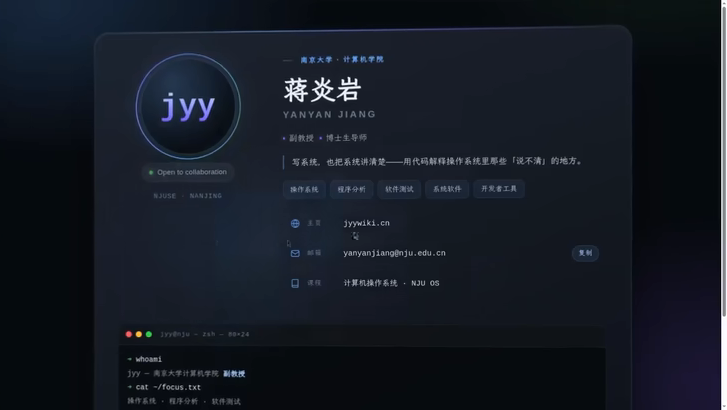
\includegraphics[width=0.98\textwidth,height=0.42\textheight,keepaspectratio]{figures/fig_11_oneshot_card.png}
\caption{一次生成的名片含错误邮箱与身份\vtag}
\end{figure}
\srcnote{00:36:30--00:36:45}
\begin{figure}[H]
\centering
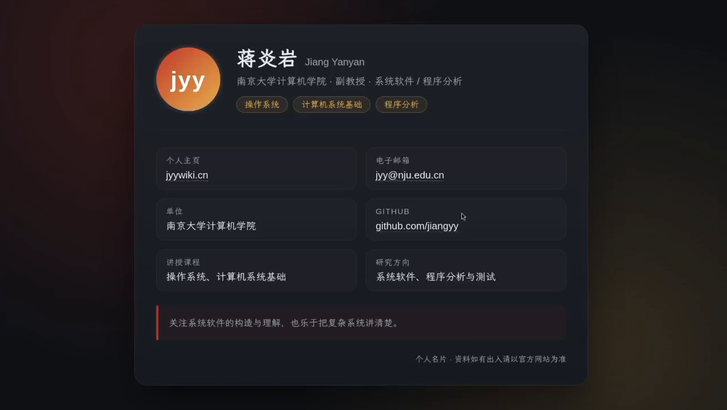
\includegraphics[width=0.98\textwidth,height=0.42\textheight,keepaspectratio]{figures/fig_12_loop_card.png}
\caption{循环生成的名片核对了邮箱与GitHub\vtag}
\end{figure}
\srcnote{00:37:30--00:37:45}

讲者同时强调输出有随机性，循环的提示词也影响结果。这次演示支持“循环与反馈能改变产物”这一观察，不能证明所有循环都更准确，更不能推出某一种模型或界面风格的普遍排名。事实核对和视觉偏好必须分别判断。

\begin{warningbox}{无限循环没有自己的验收判断}
while true 不会识别完成、停滞或预算用尽。完成标记可能被错误输出，持续修改也可能越来越偏。实际流程要约定验收条件、停止条件与重复失败后的处置；否则消耗更多 Token 可能只得到更多文件。
\end{warningbox}

\subsection{本章小结}
外层循环把一次性生成变成可接续的小步工作。它通过文件保存进展，通过版本管理记录变化，通过验收决定何时结束。每一步是不是更接近目标，还需要一套独立于开发者自信的检查。

\section{怎样让检查真正拦住错误改动}
\label{sec:ci}
持续集成与交付可以从一个朴素问题理解：工作区变了以后，怎样判断这次变化允许进入主干、交给用户？把“状态是好的”写成可执行条件，就能在每次迁移时检查，并在失败时停止后续动作。

\subsection{小步修改，让检查结果容易解释}
开发者经常觉得“只改一点点，不会出问题”。课堂用人类和 Agent 的共同倾向解释为何不能依赖这种自信。改动越小，失败时需要怀疑的范围通常越小；每轮推进后立即验证，也能在模型漂移尚未积累成大量代码前发现问题。

\begin{figure}[H]
\centering
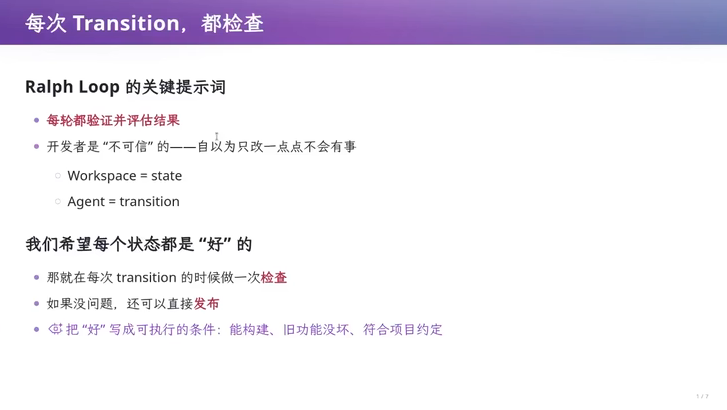
\includegraphics[width=0.98\textwidth,height=0.42\textheight,keepaspectratio]{figures/fig_13_transition_checks.png}
\caption{每次状态迁移都验证结果\vtag}
\end{figure}
\srcnote{00:42:30--00:42:45}

\begin{importantbox}{把好状态写成具体条件}
能构建、已有功能没有被破坏、项目约束得到满足，是不同的检查目标。团队先确定需要守住的条件，再选择构建、测试、静态检查或评审去判断。绿色状态的含义取决于实际运行了哪些检查。
\end{importantbox}

\subsection{持续集成与两种持续发布方式}
持续集成强调频繁把小规模修改集成到共同主干，并自动构建和验证。持续交付让软件保持可发布状态，上线时间仍可由人决定。持续部署把通过检查的变更自动发布给用户。这三个概念在课件中被并列说明。

\begin{figure}[H]
\centering
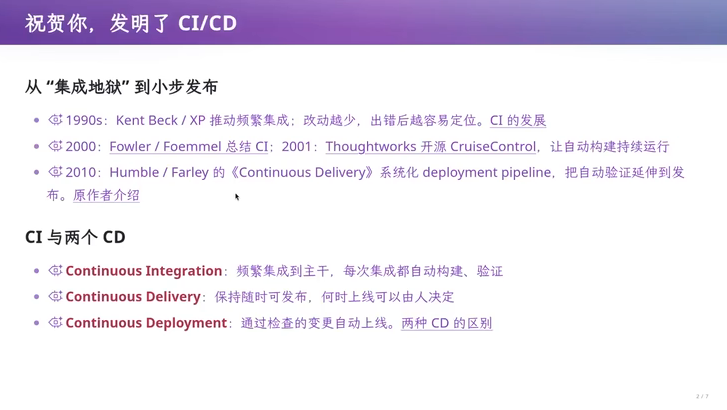
\includegraphics[width=0.98\textwidth,height=0.42\textheight,keepaspectratio]{figures/fig_14_ci_cd.png}
\caption{持续集成、持续交付和持续部署\vtag}
\end{figure}
\srcnote{00:44:30--00:44:45}

\begin{center}
\begin{tabular}{p{3.3cm}p{6.0cm}p{4.3cm}}
\toprule
流程 & 自动化承担的动作 & 是否自动上线 \\
\midrule
持续集成（CI） & 集成改动、构建、验证 & 不由名称保证 \\
持续交付（Delivery） & 维持可发布产物与交付流程 & 可保留人的决定 \\
持续部署（Deployment） & 通过检查后发布变更 & 是 \\
\bottomrule
\end{tabular}
\end{center}

课堂口头用约 20 年前概括这一发展背景，课件列出的时间更具体：1990 年代的频繁集成实践，2000 年的 CI 总结，2001 年的 CruiseControl，以及 2010 年的《Continuous Delivery》。这些是机制发展的脉络，不是今天采用 CI 就已经证明质量的理由。

\subsection{事件发生时，执行指定动作}
提交、推送、发起合并请求、合入主干都可以成为事件。Hook 指在这些事件发生前后执行约定动作。声音提醒与自动运行 Lint 使用同样的事件思路，区别在于动作内容及失败后果。团队应先说清在哪个事件运行什么，再让 Agent 编写平台配置。

\begin{figure}[H]
\centering
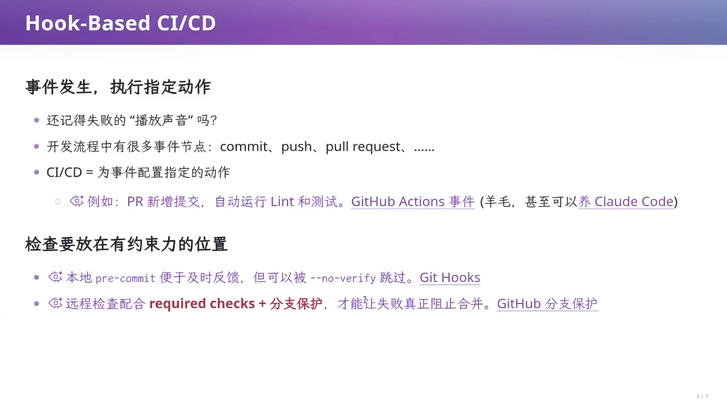
\includegraphics[width=0.98\textwidth,height=0.42\textheight,keepaspectratio]{figures/fig_15_hooks.png}
\caption{事件钩子与有约束力的合并检查\vtag}
\end{figure}
\srcnote{00:48:30--00:48:45}

本地 pre-commit 能很快反馈，但可以被跳过。远端检查只有配合必须通过的状态检查与分支保护，才可能阻止失败改动合并。这一区分使“写了检查脚本”与“流程真的有门控”成为两项验收。

\subsection{发布规则要写到失败路径}
两个 PR 单独通过，合起来可能失败；测试可能偶尔失败；线上修复可能需要例外放行；旧的发布任务还可能比新的任务晚结束，覆盖已经上线的新版。这些条件都应进入流程规格，不能靠配置文件的存在来保证。

\begin{figure}[H]
\centering
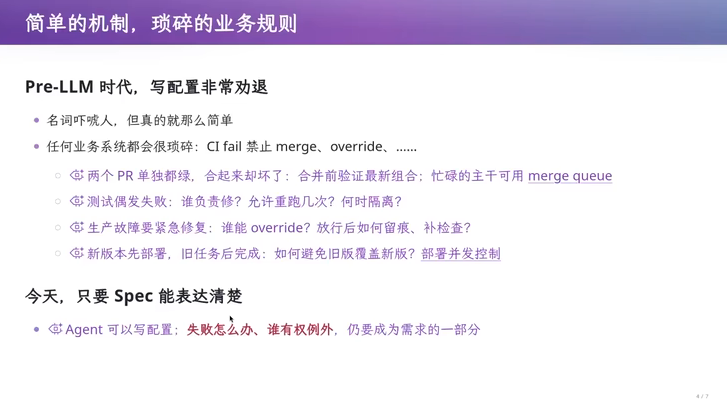
\includegraphics[width=0.98\textwidth,height=0.42\textheight,keepaspectratio]{figures/fig_16_release_rules.png}
\caption{合并组合、偶发失败与发布顺序\vtag}
\end{figure}
\srcnote{00:52:30--00:52:45}

\begin{warningbox}{验收要看门是否真的关得住}
课堂建议故意触发 Lint 或测试失败，观察合并与发布是否被阻止，再修复错误确认正常路径恢复。还要说明谁能例外放行、留下什么记录，以及重叠发布怎样处理过时产物。只观察成功运行，会漏掉门控最主要的职责。
\end{warningbox}

\subsection{本章小结}
CI/CD 把开发状态的判断安排到确定事件，并让失败改变流程。Agent 可以生成配置，团队仍需决定失败、例外和集成组合的语义。检查接下来还能用于约束维护方式，使快速生成的代码保持可读、可改。

\section{怎样把工程品味变成约束和反馈}
\label{sec:constraints}
Agent 生成得快，也可能积累得快。课堂讨论的维护负担包括文档过长、过度解释、在无关细节上反复加固，以及人难以理解的代码。想让人和 Agent 共同维护项目，需要把可判定的问题拦住，并为无法机械判定的设计保留评审。

\subsection{文档为何会成为另一份需要维护的实现}
代码之外再写一份逐行解释，会建立隐含关系：代码变了，解释也必须变。文件系统中的两个文件却不会自动提示这个关系。换一个 Agent 或压缩上下文以后，修改者可能只看见代码，留下过时文档。信息重复越多，需要同步的位置就越多。

课堂用 20K 文档举例，课件表中写为 20 KB。这里表达的是读者和维护者的负担，没有给出统一的文件容量标准。让 Agent 写得短，也不能保证它已经把重要关系讲清楚。

\begin{figure}[H]
\centering
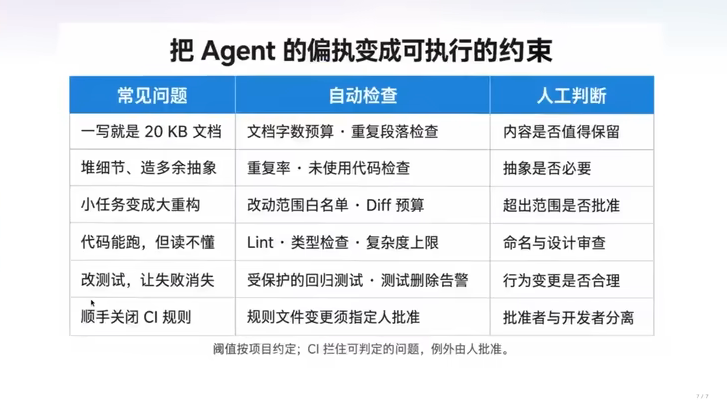
\includegraphics[width=0.98\textwidth,height=0.42\textheight,keepaspectratio]{figures/fig_17_constraint_table.png}
\caption{常见Agent偏执、自动检查与人工判断\vtag}
\end{figure}
\srcnote{00:57:30--00:57:45}

\begin{importantbox}{自动检查与人工判断各有对象}
字数、重复段落、禁止的依赖方向、代码复杂度、测试删除和规则文件变更，可以设计机械检查。内容是否值得留下、抽象是否必要、行为变化是否合理，以及例外是否批准，仍需结合项目目标判断。
\end{importantbox}

\subsection{让失败给出可以行动的信息}
课堂举例为特定文档设置 1000 字上限，后面也口头提到 1600 字的约定。这是说明“可判定规则”怎样工作，不能把两个示例合并成一条统一规范。检查读入文件长度，超过预算就失败；Agent 看到结果后压缩或重新组织文档，再按相同规则验证。

文档预算之外，依赖检查可以禁止某类模块越过架构边界。失败报告应指出违规位置与允许的访问方式，让下一轮直接处理问题。只有红叉而没有原因，会让 Agent 猜测规则。反馈要进入开发循环，才能改变下一步行动。

\subsection{知识可发现，程序行为也要可观察}
Harness 可以理解为让模型在某个项目中工作的配套环境：工具、约束、知识组织与反馈。课堂引用 OpenAI 的 Harness engineering 经验，把人的工作转向环境与流程建设。入口文档负责导航，设计、计划和决定进入版本管理，细节按需要加载。

\begin{figure}[H]
\centering
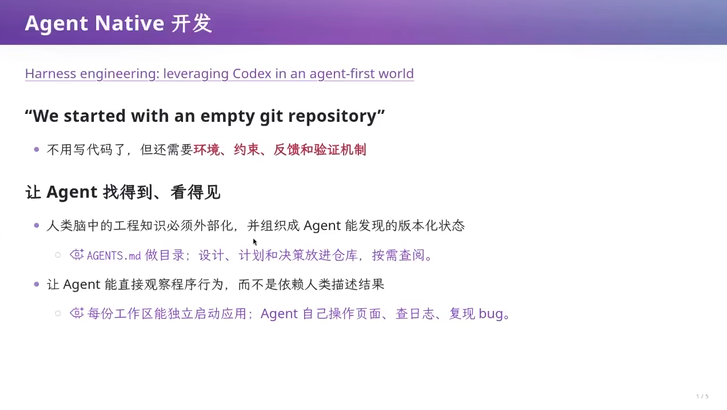
\includegraphics[width=0.98\textwidth,height=0.42\textheight,keepaspectratio]{figures/fig_18_harness_environment.png}
\caption{工程知识外部化与直接观察程序\vtag}
\end{figure}
\srcnote{01:00:00--01:00:15}

Agent 还应能够观察应用。独立工作区能启动实例，操作页面、查看日志并复现问题，就少了一层依赖人转述的反馈。这里需要的是能观察到具体行为的工具链；自动截图本身不等于已经解释了错误。

\subsection{持续清理，防止坏例子继续扩散}
代码生成会参考现有模式。一个不合适的模式留在仓库里，可能成为下一轮生成的样板。课堂因此讨论把架构要求变成检查，并持续提交小规模清理。持续修复让后来的 Agent 读到更合适的例子，也让维护负担在积累早期就被发现。

\begin{figure}[H]
\centering
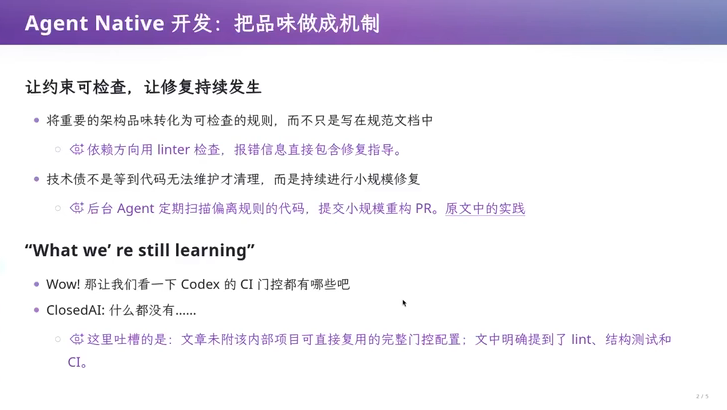
\includegraphics[width=0.98\textwidth,height=0.42\textheight,keepaspectratio]{figures/fig_19_architecture_rules.png}
\caption{可检查的架构约束与持续清理\vtag}
\end{figure}
\srcnote{01:03:30--01:03:45}

\begin{warningbox}{实现者不能为了变绿，单方面降低标准}
删除失败断言、关闭 CI 或放宽规则，也能让检查显示成功。需要修改规则时，应回到原先的需求与设计理由，并按约定批准。修复了行为与取消了判断，不能在验收中混为一谈。
\end{warningbox}

课件对 OpenAI 未公开完整内部配置的讨论，只支持“文章经验不能直接等同于可复制的整套实现”。文章确实介绍了 Lint、结构测试和 CI；讲者关于更深层内部机制的判断，不构成对未公开系统的验证。

\subsection{本章小结}
可机械判定的维护要求应成为可运行规则，规则还应解释失败与修复方向。知识入口和可观察应用缩短反馈路径，人工评审负责目标和品味。并行增加以后，同样需要检查反馈能否分解任务。

\section{多个 Agent，怎样避免同时修同一个问题}
\label{sec:parallel}
并行收益取决于任务能否分开推进。开更多进程只增加执行者；如果所有人看到相同的失败入口，仍可能重复工作并覆盖彼此。课堂的编译器案例说明，验证方法本身能改变任务是否可分。

\subsection{失败太粗，任务就挤在同一个入口}
课堂介绍 Anthropic 的 C 编译器实验：16 个 Agent 协作，在编译 Linux 时先撞上同一个错误，重复修复并相互覆盖。这里的瓶颈是反馈只暴露了一个整体失败。增加执行者没有增加独立问题，协调反而更困难。

\begin{figure}[H]
\centering
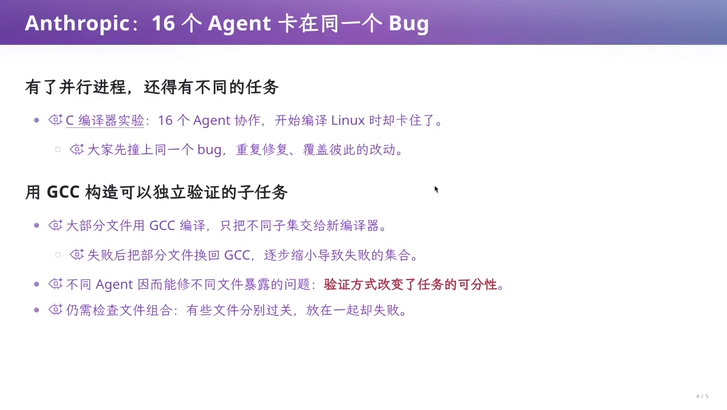
\includegraphics[width=0.98\textwidth,height=0.42\textheight,keepaspectratio]{figures/fig_20_compiler_parallel.png}
\caption{16个Agent及GCC划分验证子集\vtag}
\end{figure}
\srcnote{01:05:00--01:05:15}

\begin{importantbox}{先检查工作能否独立验收}
任务划分应回答：每个 Agent 修改什么、依赖什么、怎样判断自己完成，以及组合后还要检查什么。同一个失败日志不能自动变成多个不同任务；有独立的观察与验收入口，才有机会并行推进。
\end{importantbox}

\subsection{可信参照，怎样缩小失败集合}
案例用 GCC 编译大部分文件，只让新编译器负责一部分。失败后把部分文件换回 GCC，继续缩小导致问题的文件集合。这样，不同 Agent 能面对不同子集暴露的问题。验证由“整个内核失败”变成“这个子集仍失败”，任务表示就细了。

单独能编译的文件放在一起，仍可能出现交互错误，所以子集验证之后还要检查组合。GCC 在这里帮助隔离问题。课堂用这个例子说明，验证应提供能划分任务的反馈；编译成功之后，仍需检查其他功能和文件组合。

\subsection{总负责人需要看见任务与模块的关系}
讲者分享自己的项目组织方式：架构文档生成图，任务簿记录工作状态，正在推进的任务显示在相应模块上。负责人可以观察哪些 Agent 在哪些模块工作，再决定任务安排与架构调整。估计进度条帮助调度，实际完成仍需对应产物与检查结果。

这种表示把“某个窗口还在跑”变成“这个模块在处理哪件事”。如果同一个模块出现互相冲突的任务，负责人就有机会提前协调。若所有状态只藏在聊天窗口中，负责人很难恢复整个项目的依赖和进展。

\subsection{调度也可以使用不同类型的动作}
同一份工作区可以交给实现 Agent、评审 Agent 或重构 Agent。不同动作探索设计空间的不同方向：实现推进一个方案，评审判断风险，重构改变结构。讲者还讨论由主 Agent 分配任务的可能性，并说明自己仍在尝试。这部分是一种工作流设计方向，没有证明全自动调度可以替代人的架构判断。

\begin{warningbox}{进度可见，不等于集成已通过}
任务状态与进度估计供协调使用。验收还要确认对应提交、独立检查和集成结果。两个分支各自通过时，不能据此宣告合在一起已经正确。
\end{warningbox}

\subsection{本章小结}
并行先需要任务可分，再需要状态可见，最后需要组合验收。可信参照和可缩小的失败集合能创造独立任务，架构图与任务簿能帮助协调。项目中的文档关系也需要从隐含约定变成这种可检查的表示。

\section{两种语言的文档，怎样保持同一件事}
\label{sec:bilingual}
课堂对 DeepSeek Harness 的现场阅读，重点放在一个具体维护问题：中文与英文都需要让人容易读，但每次修改以后，两份文档仍应表达同一件事。把两份文件摆在同一目录，只能说明位置相近，不能保证同步。

\subsection{文件之外，还需要表示关系}
课堂展示的架构文档包含交叉引用和模块关系。一个项目里的信息并非互不相关的文件集合：某段文字解释接口，另一份文字翻译它，还有决定记录说明为何采用它。让 Agent 可靠维护这些信息，需要把关系表达出来。

\begin{figure}[H]
\centering
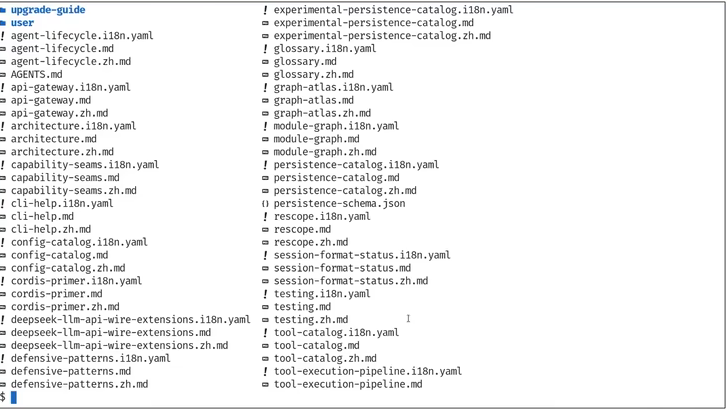
\includegraphics[width=0.98\textwidth,height=0.42\textheight,keepaspectratio]{figures/fig_21_document_pairs.png}
\caption{文档目录中的英文、中文与配对记录\vtag}
\end{figure}
\srcnote{01:09:00--01:09:15}

\begin{importantbox}{双语配对的三件套}
课堂展示每篇配对文档由英文文件、中文文件和一致性记录组成。记录按章节保存两边文本的哈希与相关约定。两种语言没有固定主次；某次修改先发生在哪一边，那一边就是这次变更的来源。
\end{importantbox}

\begin{figure}[H]
\centering
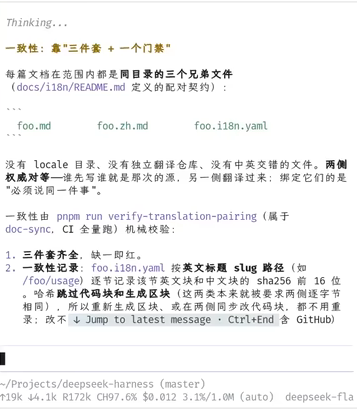
\includegraphics[width=0.98\textwidth,height=0.65\textheight,keepaspectratio]{figures/fig_22_doc_triplet.png}
\caption{双语文档三件套与同目录配对\vtag}
\end{figure}
\srcnote{01:11:00--01:11:15}

\begin{lstlisting}[caption={课堂展示的同目录文档配对形式}]
foo.md
foo.zh.md
foo.i18n.yaml
\end{lstlisting}

\subsection{哈希指出变化，结构检查寻找漂移}
哈希是对文本内容计算的摘要。当前文本与记录中的哈希不同，就能发现内容发生了变化；结合版本历史，还能比较变化先后。画面展示的记录按文档标题路径保存中英文摘要。课堂说明，标题 slug、代码围栏、表格等结构也可以参与检查。

\begin{figure}[H]
\centering
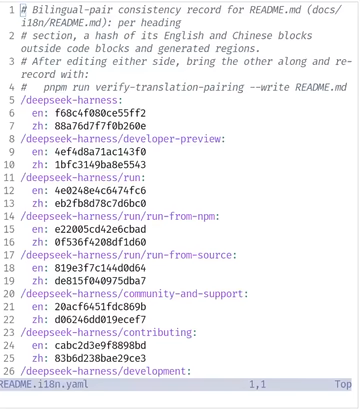
\includegraphics[width=0.98\textwidth,height=0.65\textheight,keepaspectratio]{figures/fig_23_pair_hash.png}
\caption{双语配对记录中的章节哈希\vtag}
\end{figure}
\srcnote{01:12:00--01:12:15}
\begin{figure}[H]
\centering
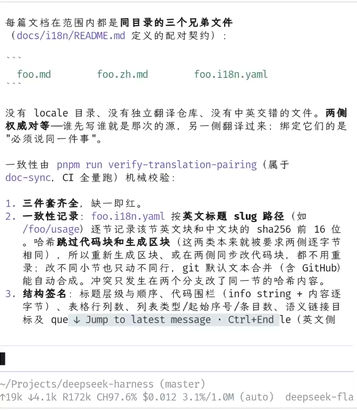
\includegraphics[width=0.98\textwidth,height=0.65\textheight,keepaspectratio]{figures/fig_24_pair_checks.png}
\caption{内容哈希、结构签名与最小补丁\vtag}
\end{figure}
\srcnote{01:14:00--01:14:15}

哈希不能证明翻译正确。它证明的是当前文本是否与记录过的文本相同。若中英文都重新写过并刷新记录，两个哈希完全匹配，语义仍可能不一致。翻译审阅与结构规则需要回答不同问题：有没有未同步的修改，关键结构有没有漂移，最后两边是否仍表达同一意图。

\subsection{最小补丁，避免整篇重写带来的变化}
课堂提出按改动部分翻译：先看源文档变了哪些段落，再修改译文对应位置，保留其余内容。整篇重新生成可能改变原先没有问题的措辞、结构和术语，增大需要审阅的范围。小补丁让审阅者能把注意力放在本次真实变化上。

三件套增加目录里的文件数量，可以用 IDE 视图隐藏暂时不需要的语言或一致性文件。隐藏只改变人的浏览视图，配对关系仍保存在仓库中。中文读者与英文读者可以得到适合自己的入口，同时共享同一套维护关系。

\subsection{人能读懂的文风，也需要可查阅的样例}
现场阅读展示了三类材料：金标准样例、术语表，以及原意写作和翻译规则。样例展示哪些段落值得模仿、哪些写法不合适；术语表给出统一译法；工作规则说明该如何修改。这些材料按任务需要加载，避免把全部规范堆入每轮上下文。

\begin{figure}[H]
\centering
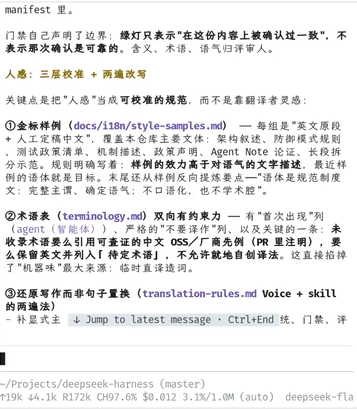
\includegraphics[width=0.98\textwidth,height=0.65\textheight,keepaspectratio]{figures/fig_25_style.png}
\caption{金标准样例、术语与翻译规则\vtag}
\end{figure}
\srcnote{01:16:00--01:16:15}
\begin{figure}[H]
\centering
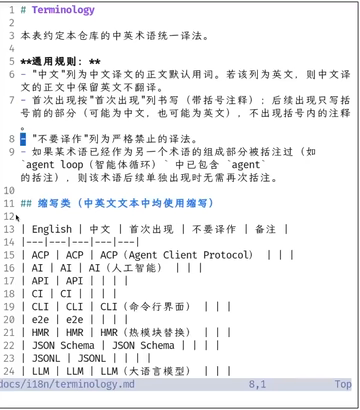
\includegraphics[width=0.98\textwidth,height=0.65\textheight,keepaspectratio]{figures/fig_26_terminology.png}
\caption{允许与禁止的中英文术语译法\vtag}
\end{figure}
\srcnote{01:16:00--01:16:15}

课堂提到，即使达到 100万 规模的上下文，也可能装不下不断膨胀的全部规范。这里的数字用于说明把知识一次性塞入会话的局限。分层入口与按需加载，是组织知识的方法，不能被误解为仅仅扩大模型窗口。

\begin{warningbox}{规则要能发现问题，也要允许合理翻译}
课堂讨论了按段落检查术语出现次数的设想，并举出加减 2--3 次的容差。这是说明决策边界需要调校的例子，不是该仓库已实施的统一阈值。中英文表达方式不同，过严计数可能拒绝正确译文，语义评审仍需保留。
\end{warningbox}

\subsection{本章小结}
双语一致性需要可见的配对、变更记录、结构规则和语义判断。哈希发现未同步内容，小补丁缩小审阅范围，样例与术语维持表达约定。下一步是让设计决定和工作方法也有明确位置与生命周期。

\section{知识怎样留在仓库里，又不会越积越乱}
\label{sec:knowledge}
可恢复的工作区不能只有代码，也不能是一份无休止增长的说明书。课堂将指令、设计决定、技能和机械门控分别展示，说明哪些知识应常驻、哪些按需查阅、哪些可以在过期后归档。

\subsection{从开发历史看设计理由，保留证据的层次}
讲者让 Agent 读取 Git 历史，还原双语一致性流程的演进。现场摘要从 2026年 6 月 10 日的初始仓库说起，列出 6 月下旬的术语约定、7 月初的配对契约与门控，以及后续最小补丁和工作流调整。下面两图是课堂生成的历史摘要。

\begin{figure}[H]
\centering
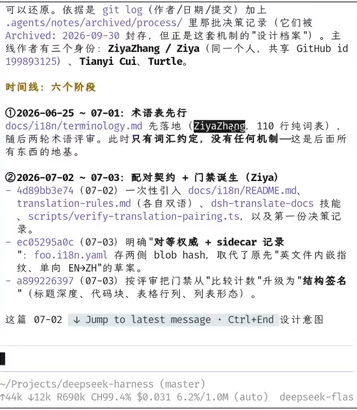
\includegraphics[width=0.98\textwidth,height=0.65\textheight,keepaspectratio]{figures/fig_27_history_early.png}
\caption{现场生成摘要中的术语与配对契约演进\vtag}
\end{figure}
\srcnote{01:19:00--01:19:15}
\begin{figure}[H]
\centering
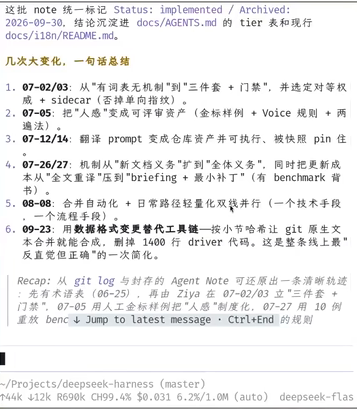
\includegraphics[width=0.98\textwidth,height=0.65\textheight,keepaspectratio]{figures/fig_28_history_late.png}
\caption{现场摘要中的最小补丁与工作流演进\vtag}
\end{figure}
\srcnote{01:20:30--01:20:45}

这些材料提供了进一步查阅提交的入口。摘要中“最小补丁”“briefing”等标签可以帮助理解机制变化，具体作者、日期与因果仍应回到相应提交核对。本讲义保留机制的演进方向，不以一段生成摘要替原仓库完成历史审计。

\begin{importantbox}{入口、决定、方法和门控承担不同职责}
入口文档指向该读哪里；决定记录说明选择与理由；技能说明怎样开展一类工作；门控把可判定约定变成会运行的检查。把四种内容全塞进一个入口，会让每一轮都承担不必要的阅读负担。
\end{importantbox}

\subsection{常驻指令要短，决策记录要有状态}
课堂展示按目录分层的 AGENTS.md，以及文档预算检查。屏幕摘要给出的阈值是根级入口文档（root）不超过 1960 词、架构说明（architecture）不超过 2400 词。自动字幕把“词”听成了“次”，这里按画面校正。阈值属于课堂所读版本的约定，不能推广为所有项目的标准。

\begin{figure}[H]
\centering
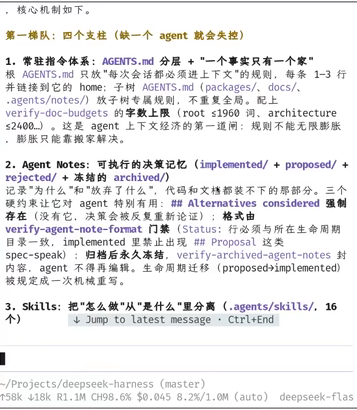
\includegraphics[width=0.98\textwidth,height=0.65\textheight,keepaspectratio]{figures/fig_29_agent_notes.png}
\caption{分层指令预算与Agent Notes生命周期\vtag}
\end{figure}
\srcnote{01:23:00--01:23:15}

Agent Notes 区分 proposed、implemented、rejected 和 archived：提案不等于已经实现，拒绝的方案仍值得保存理由，归档表示退出当前工作状态。课堂还展示格式与归档检查，使状态标签、正文要求和生命周期保持对应。保留曾考虑的替代方案，下一轮就不必重新猜为何采用当前结构。

\subsection{技能把做什么与怎么做分开}
任务计划说明目标与验收，技能提供一类工作的操作方法。课堂按流程门控、写作规范、工程质量和元技能展示分类。代码评审、错误处理、性能检查或文档翻译，可以分别使用对应方法，而不必在每个任务描述中重复整套说明。

\begin{figure}[H]
\centering
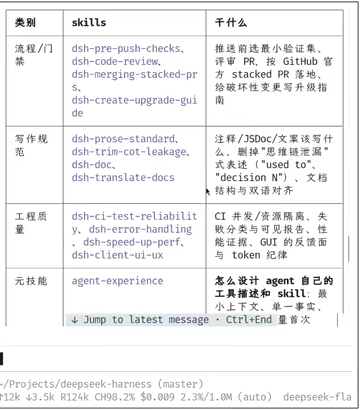
\includegraphics[width=0.98\textwidth,height=0.65\textheight,keepaspectratio]{figures/fig_30_skills.png}
\caption{流程、写作、工程与元技能的分类\vtag}
\end{figure}
\srcnote{01:24:00--01:24:15}

屏幕摘要提到 16 个技能。这个数量只是当时展示的组织规模；值得借鉴的是路由关系：什么任务触发什么材料，哪些动作由用户明确调用，哪些知识按需要读取。堆积更多技能并不自动增加判断力，入口仍要让 Agent 找到与当前任务有关的那份材料。

\subsection{接口与说明之间的关系，也能被检查}
课堂展示类型等价检查：文档中的类型或接口需要与源代码一致，防止程序接口更新而说明没有跟上。讲者进一步分享把 Markdown 代码块与某处内容关联的做法，通过轻量检查声明这段代码应出现在哪里、怎样与其他材料对应。

\begin{figure}[H]
\centering
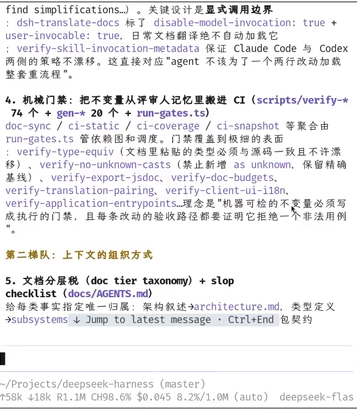
\includegraphics[width=0.98\textwidth,height=0.65\textheight,keepaspectratio]{figures/fig_31_mechanical_checks.png}
\caption{类型等价、文档同步与架构关系检查\vtag}
\end{figure}
\srcnote{01:27:00--01:27:15}

屏幕摘要列出 doc-sync、ci-static、ci-coverage 和 ci-snapshot 等检查组，并提到 74 个 verify 脚本与 20 个生成脚本。这里保留的是课堂显示的规模信息，没有执行这些脚本，不能由数量判断它们覆盖了所有风险。机制价值在于不同关系有对应检查，失败能够指向应修的位置。

\begin{warningbox}{内容来自同一个位置，不保证内容本身正确}
从注释生成 API 文档，可以减少独立复制导致的漂移；检查文档代码与源码一致，可以验证两份材料对应。注释可能过时，接口设计也可能不合理，机械一致性仍需与行为测试和设计评审结合。
\end{warningbox}

\subsection{本章小结}
知识留在仓库里，需要入口、关系和生命周期。常驻指令有预算，决定有状态，技能有任务入口，接口说明有检查。这样下一轮 Agent 读取的是可用的当前知识，同时还能追溯过去的选择。

\section{什么时候应当改变架构，以及怎样获得这种判断}
\label{sec:refactor}
持续清理能修复重复、过时说明和违反规则的代码，但有些问题来自整个系统的前提。当前提失效，继续把局部整理得更漂亮，也不会改变负载、需求或协作结构。课堂把这一边界连接到重构与实践经验。

\subsection{清理技术债，不能代替重新设计}
课堂把日常清理类比为垃圾回收：发现并移除不良模式，修复文档，减少重复。这是维护活动的类比，并非运行时内存管理。若数据组织或模块职责已不适合目标，清理只能维持原结构。讲者分享的办法是开一份新的结构，逐步迁入旧功能，让重构后的功能继续接受检查。

\begin{figure}[H]
\centering
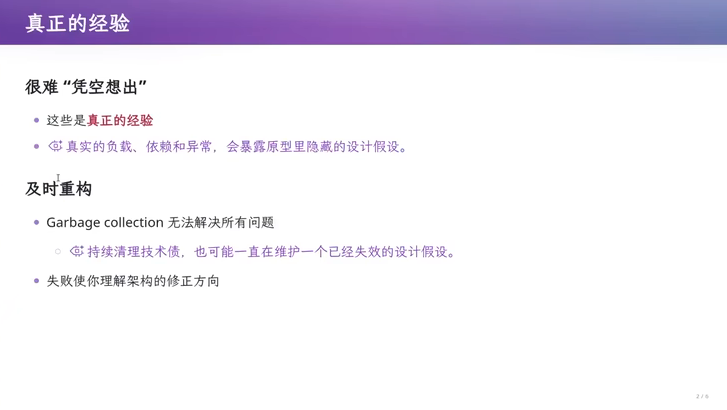
\includegraphics[width=0.98\textwidth,height=0.42\textheight,keepaspectratio]{figures/fig_32_refactor.png}
\caption{持续清理的边界与架构重构\vtag}
\end{figure}
\srcnote{01:29:30--01:29:45}

\begin{importantbox}{失败应当改变下一轮的选择}
当相同架构前提反复导致问题，应重新讨论前提，而不只增加补丁。重构可以发生在模块或项目层面。迁移哪些功能、保留哪些行为、怎样验证，都应回到规格与验收。
\end{importantbox}

\subsection{Friendster：技术瓶颈与组织实施是两道关}
课件介绍单主库加多个完整副本的结构。增加读副本能分担读取，但每个副本仍要重放全部写入，复制与 I/O 压力可能增加延迟。按用户分片则让不同服务器承担不同数据与对应负载，改变了原先所有副本都承受完整更新的前提。

\begin{figure}[H]
\centering
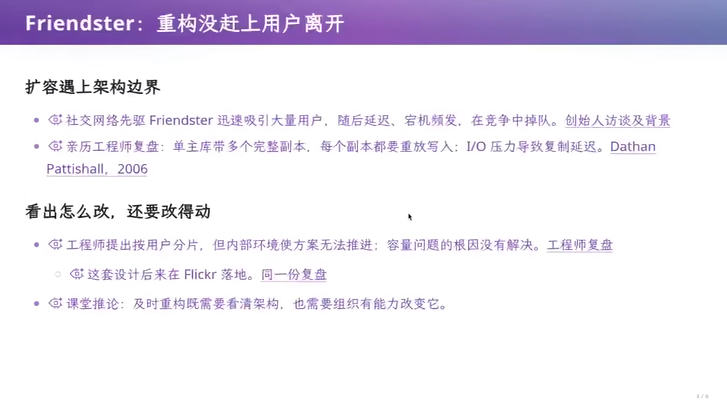
\includegraphics[width=0.98\textwidth,height=0.42\textheight,keepaspectratio]{figures/fig_33_friendster.png}
\caption{复制写入瓶颈、用户分片与组织实施\vtag}
\end{figure}
\srcnote{01:30:30--01:30:45}

课件引用工程师的 2006 年复盘，说明分片方案没有在 Friendster 顺利推进，后来在 Flickr 落地。这是亲历者的复盘，能够说明技术方案与组织执行之间的落差，不能单独解释一家公司的全部兴衰。看懂应该怎样改，还需要组织能安排数据迁移、工作分配和上线过程。

\subsection{实现便宜以后，需求假设仍可能失败}
Webvan 和 Quibi 在课件中作为产品假设的案例。Webvan 的仓配能力与订单密度没有同步：课件引用 2000 年年报，配送中心负载不足设计容量的 40\%，并列出 2001 年 7 月申请破产。
Quibi 的 2020 年告别信把独立服务的需求与推出时机列为可能原因。

\begin{figure}[H]
\centering
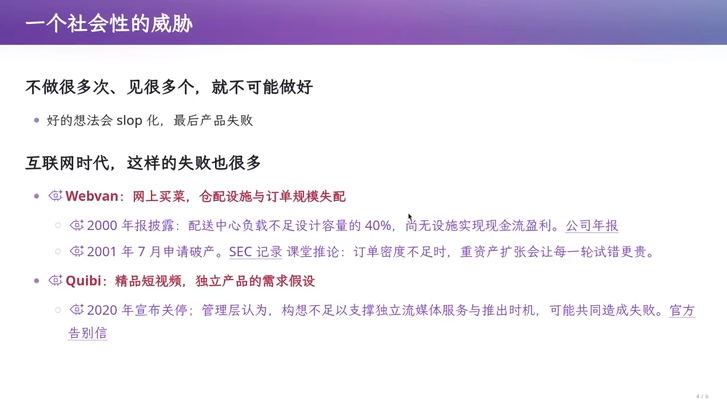
\includegraphics[width=0.98\textwidth,height=0.42\textheight,keepaspectratio]{figures/fig_34_business_cases.png}
\caption{Webvan与Quibi的需求假设\vtag}
\end{figure}
\srcnote{01:31:00--01:31:15}

这些案例提示读者区分“可以实现”与“值得以这种规模实现”。仓配设施会放大未验证需求的成本；精品短视频内容存在，也不保证用户需要一个独立服务。Agent 能快速生成页面和功能，仍需要运行结果、使用场景和真实反馈来检验假设。

\subsection{实践机会，会影响工程判断怎样形成}
讲者最后讨论学习资源。见过不同系统、自己做过修改并读懂失败反馈，才能比较哪些约束有用、哪些只是噪声。Token 预算代表部分试错资源，没有同样的实践机会，就可能积累不同的经验。开源项目提供观察材料，亲手运行仍能带来仅靠阅读不容易获得的反馈。

\begin{figure}[H]
\centering
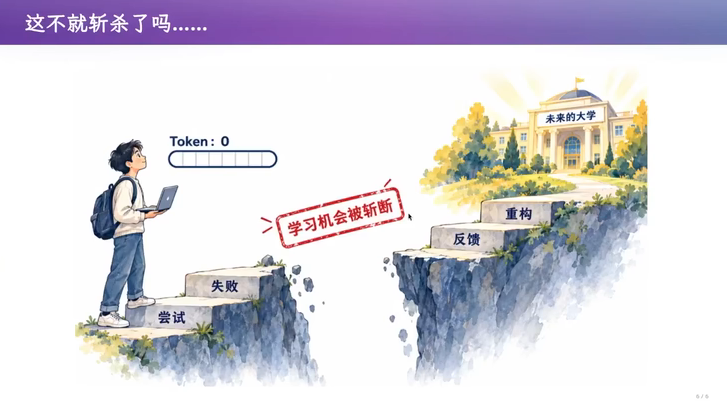
\includegraphics[width=0.98\textwidth,height=0.42\textheight,keepaspectratio]{figures/fig_35_learning_access.png}
\caption{Token资源与实践机会之间的关系\vtag}
\end{figure}
\srcnote{01:35:30--01:35:45}

课堂提到 4年 或五年的培养周期、20美元 的个人订阅，以及用 1000万 争取优秀课程设计人才的设想。前两项分别用于讨论培养回报与讲者个人使用体验，后一项是教育组织形态的假设表达，均没有给出可普遍比较的评估样本。不能把这些口述数字当作今天的产品价格建议、统一人才价值或已经发生的教育投入。

\begin{warningbox}{关于教育与就业，保留判断的身份}
讲者担忧实践资源差距和企业追求即时产出，会改变初学者得到训练的机会。这是课堂提出的社会风险和未来判断，没有证明某一代人必然被替代。资源之外，愿意理解反馈、比较方案并组织下一轮尝试，同样影响学习结果。
\end{warningbox}

\subsection{本章小结}
重构改变系统的前提，清理改善现有结构，二者解决不同问题。判断来自能够改变下一步行动的失败与比较。学习者需要实践机会，也需要把一次尝试留下的经验变成下一轮可验证的改进。

\section{总结与延伸}
\label{sec:synthesis}
本讲可以压缩成一个开发闭环：明确当前要做什么，读取可恢复的工作区，推进一小步，检查行为和约束，再把结果与下一步留回工作区。内循环负责工具调用，外循环负责任务接续，CI 门控负责让失败产生后果。文档配对、接口关系和决定记录，让不同轮次看到一致的工程知识。

\subsection{讲者的结论，与这份讲义的整理}
讲者建议通过真正做过的系统与开源项目学习 Agent-native 开发，关注项目怎样处理约束、反馈和失败。DeepSeek Harness 的现场阅读展示了很多细小关系如何被表示和检查。课堂同时提醒，持续清理不能解决全部问题，必要时要回到设计空间改变架构。

本讲义据此将人的责任整理为三项：表达目标与验收，判断哪些约束值得固定，以及在反馈显示前提失效时选择新的结构。Agent 能执行大量具体工作，人的判断通过规格、方法和门控进入过程。留下可检查的结果，比要求模型“做得好一点”更容易成为下一轮的行动依据。

\begin{importantbox}{把课程用于自己的项目}
选择一个现有小任务，写清完成条件与状态文件；安排一次工具执行和一次结果回写；为一项经常漂移的关系设置检查。用失败触发检查，再确认修复后正常流程恢复。每项练习都应留下观察结果，便于比较下一轮修改。
\end{importantbox}

\subsection{怎样检查自己是否理解了闭环}
读者可以用课堂中的名片任务开始：分别检查页面能否打开、公开资料是否正确、视觉效果是否符合需要。再用双语文档练习同步：修改一边，观察配对检查怎样报告另一边需要更新，审阅最小补丁，确认语义仍一致。并行练习则要比较分支各自通过与合并后通过，看到两种验收对象的差别。

这些练习沿用课堂出现的任务与失败边界，是本讲义的教学整理。它们没有构成新的性能实验，也不会仅因多运行几轮就证明哪种模型更好。课堂演示回答的是机制如何运转；项目采用以后，还需要对自己的任务和约束验收。

\begin{warningbox}{保留证据的范围}
名片对照是现场演示；仓库结构与开发历史包含现场生成摘要；产品窗口与订阅是授课时的观察；社会影响是讲者判断。读者可以由这些材料提出下一步检查，但不应把它们合并成已经完成的普遍质量证明。
\end{warningbox}

\subsection{口述数字的阅读边界}
字幕中的一些数字只是修辞或背景。07:50 的“10万 八千里”形容路线差别，没有测量结果；11:27 的 2023年 是课堂回顾听众接触聊天式 AI 的时间；51:37 的 2000分钟 是讲者带有“好像”的 CI 资源回忆；56:39 的 10亿 只狗来自讲者转述的超级智能类比，没有在本课核查种群统计。这些数字不作为本讲义的技术结论或当前服务规格。

\subsection{本章小结}
可持续开发的判断落在具体变化上：状态能恢复，检查会拦住失败，信息关系能跟上修改，必要时能改变架构。下一次尝试的价值，来自它让我们知道应该继续哪条路、修复什么，以及哪些问题仍然没有证据。

%% --- 正文内容结束 --- %%

\end{document}
